\newtheorem{definition}{Định nghĩa}[section]    
\newtheorem{theorem}{Định lý}
\newtheorem{corollary}[theorem]{Hệ quả}
\newtheorem{lemma}[theorem]{Bổ đề}

%%Khái niệm
\section{Hàm Số}    
\begin{definition}
Hàm $f$ là một quy tắc cho tương ứng mỗi phần tử $x$ thuộc tập hợp $X$ với một và chỉ một phần tử, kí hiệu $f(x)$, thuộc tập hợp $Y$.
\end{definition}    
\begin{itemize}
    \item $X$ được gọi là tập hợp (miền) xác định của hàm $f$.    
    \item $Y$ được gọi là tập hợp giá trị của hàm $f$. 
    \item Nếu $X$ và $Y$ là tập các số thực, khi đó hàm được gọi là hàm số.
\end{itemize}

\begin{figure}[htbp]
    \centering
    \includegraphics[width=8cm, height=5cm]{Tuan1/ảnh/anhxa.png}\label{anh1.1}
\end{figure}
\subsection{Đồ thị hàm số}
Hàm số có thể được biểu diễn bằng công thức, bảng, đồ thị hoặc mô tả bằng lời nói. Trong đó trực quan nhẩt là biểu diễn thông qua đồ thị. 
\begin{definition}
    Đồ thị của hàm số $f$ có miền xác định $X$ là tập hợp các cặp có thứ tự  \[ \{\left(x,f(x)\right)\vert x\in X \} .\] 
\end{definition}
Nói cách khác, đồ thị của $f$ bao gồm mọi điểm $(x,y)$ sao cho $y=f(x)$ với $x\in X$
\begin{figure}[htbp]
    \centering
    \begin{subfigure}{0.4\textwidth}
        \centering
        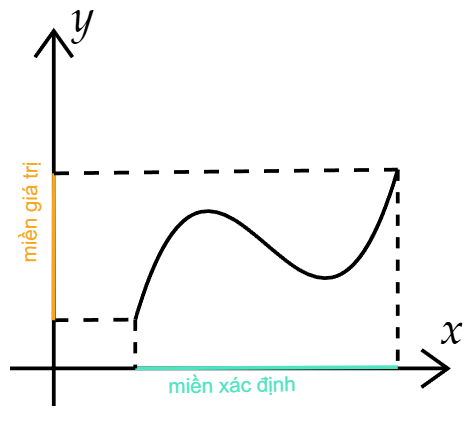
\includegraphics[width= 0.8\linewidth]{Tuan1/ảnh/hamso1.png}
        \caption{}
    \end{subfigure}
    \hfill
    \begin{subfigure}{0.4\textwidth}
        \centering
        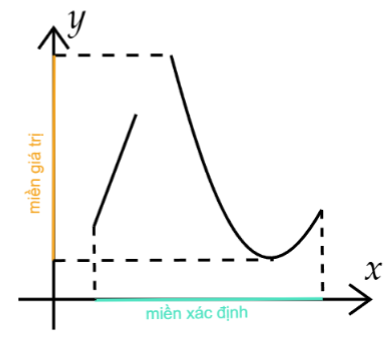
\includegraphics[width=0.8\linewidth]{Tuan1/ảnh/hamso2.png}
        \caption{}
    \end{subfigure}
    \caption{Ví dụ về đồ thị hàm số}\label{anh1.2}
    \end{figure}

Các điểm này có thể là vô số, tạo thành những đường cong hoặc đường thẳng trên mặt phẳng, liên tục hoặc rời rạc. Song không phải mọi đường bất kỳ đều là đồ thị của một hàm số nào đó. Để là đồ thị của một hàm số, mỗi hoành độ $x$ phải tương ứng với một tung độ $y$ duy nhất. Nghĩa là không được có hai điểm khác nhau trên đồ thị có cùng hoành độ nhưng khác tung độ.

Một cách trực quan,\emph{ không có đường thẳng thẳng đứng (vuông góc với trục hoành) nào cắt đồ thị của một hàm số nhiều hơn một lần.} (xem \ref{anh1.2})
\begin{figure}[htbp]
    \centering
    \begin{subfigure}{0.4\textwidth}
        \centering
        \includegraphics[width= 7cm, height=6cm]{Tuan1/ảnh/hamsochuan.png}
        \caption{Đồ thị hàm số}
    \end{subfigure}
    \hfill
    \begin{subfigure}{0.4\textwidth}
        \centering
        \includegraphics[width=7cm, height=6cm]{Tuan1/ảnh/khongphaihamso.png}
        \caption{Không phải đồ thị hàm số}
    \end{subfigure}
    \caption{So sánh}\label{anh1.3}
    \end{figure}

%%%Các hàm
\subsection{Các hàm thông dụng}

Trong khi xử lý các bài toán, chúng ta thường gặp các hàm số có dạng tổng quát. Các hàm này được phân loại theo dạng biểu thức của chúng. Dưới đây là một số loại hàm số cơ bản:   \begin{itemize}
    \item Hàm \emph{tuyến tính} có dạng $f(x) = ax + b$, với $a$ và $b$ là các hằng số. Đồ thị của hàm tuyến tính là một đường thẳng.\newline Ví dụ: $ 2x+3$.
    \item Hàm \emph{đa thức} có dạng $P(x) = a_n x^n + a_{n-1} x^{n-1} + \ldots + a_1 x + a_0$, với $a_n, a_{n-1}, \ldots, a_0$ là các hằng số và $n\in\mathbb{N}$ là bậc của đa thức.\newline Ví dụ: $x^2 - 4x + 4; x^5 + 2x^2 - 5x + 1$; $3x+2$.
    \item Hàm \emph{luỹ thừa} có dạng $f(x)=x^\alpha$, với $\alpha\in\mathbb{R}$ là một hằng số.\newline Ví dụ: $x^2, x^{-3}=\frac{3}{x}, x^{5/2}=\sqrt{x^5}=(\sqrt x)^5$.     
    \item Hàm tỷ lệ có dạng $f(x) = \frac{P(x)}{Q(x)}$, với $P(x)$ và $Q(x)$ là các đa thức. Ví dụ: $\frac{x^2+1}{x-2}$.    
\end{itemize}
Trên đây được gọi chung là các hàm \emph{đại số}, tức là các hàm có thể được biểu diễn bằng các toán tử đại số như cộng, trừ, nhân, chia và lũy thừa.\newline
Ví dụ : $\frac{\left(x^5+x^3-x^2+4\right)^{3/2}}{x+\sqrt x}$.
\vspace{8pt}

Ta cũng liệt kê thêm một số hàm không thuộc loại trên.\newline
Ví dụ như các hàm \emph{siêu việt}:\begin{itemize}
    \item Hàm \emph{lượng giác} là các hàm $\sin x,\cos x, \tan x, \dots$ mà có thể được định nghĩa thông qua các điểm trên một đường tròn đơn vị.
    \item Hàm \emph{mũ} và \emph{lôgarit} lần lượt có dạng $f(x) = a^x$ và $f(x) = \log_a x$, với $a > 0$ là một hằng số. Cái sau là hàm \emph{nghịch đảo} của cái trước, tức là $\log_a a^x = x$ và $a^{\log_a x} = x$.\newline Ví dụ: $2^x \text{ và } \log_2 x$; $e^x \text{ và } \ln x$.
\end{itemize}
Hay, hàm xác định từng phần là các hàm được xác định bởi các công thức khác nhau trên các miền khác nhau của tập xác định.\newline
Ví dụ, hàm giá trị tuyệt đối $f(x) = |x|$ được định nghĩa:
\begin{equation*}
    f(x) = \left\{
\begin{aligned}
x  & \quad \text{nếu } x \geq 0 \\
-x   & \quad \text{nếu } x < 0
\end{aligned}
\right\}.
\end{equation*}

Trong tất cả những hàm vừa liệt kê lại có một số hàm có tính chất chung. Chẳng hạn như tính chẵn lẻ, tính đồng biến nghịch biến, tính liên tục,...\newline
Trước khi sang phần tiếp theo, hãy nói qua thêm một khái niệm nữa, đó là \emph{hàm hợp}. Ta biết rằng hàm số là một thứ mà ta cho vào một giá trị và sẽ cho ra một giá trị nào đó. Trên cơ sở này, hàm hợp là một hàm số mà đầu vào của nó là đầu ra của một hàm số khác.\newline
Xét hai hàm $f(x)$ và $g(x)$, hàm hợp của chúng được ký hiệu là $f(g(x))$ và được đọc là "hàm $f$ của hàm $g$ tại $x$". Hàm hợp này sẽ nhận đầu vào là giá trị của hàm $g(x)$ và trả về giá trị của hàm $f$ tại điểm đó.\newline    
Ví dụ: $f(x)=x^2$, $g(x)=\sin x$ vậy $f(g(x))=f(\sin x)=\sin^2 x$.
\section{Giới Hạn Hàm Số}
\subsection{Ví dụ về giới hạn}
Xét hàm số $y=x^2$, phóng to đồ thị vào gần điểm $(1;1)$:
\begin{figure}[h!]
    \centering
    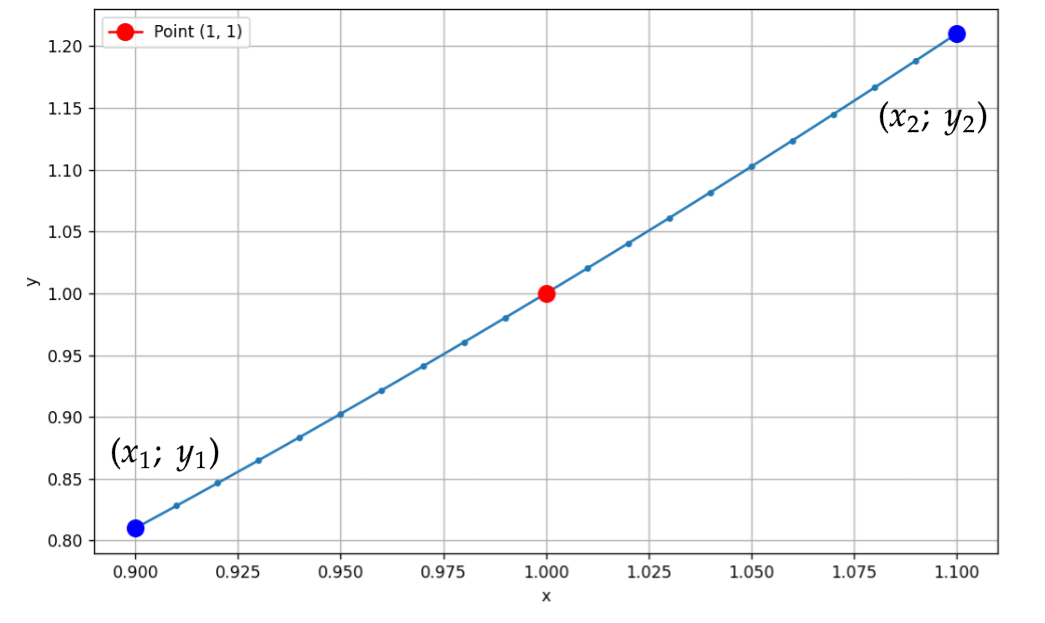
\includegraphics[width=0.6\textwidth]{Tuan1/ảnh/0.9-1.1.png}
    \caption{Đồ thị \(y=x^2\) được phóng to trong khoảng $[0.9;1.1]$}
    \label{anh3}
\end{figure}

Hãy tưởng tượng có hai con bọ xuất phát từ hai điểm xanh và bò lại \emph{gần} điểm màu đỏ trên con đường tạo thành từ đoạn đồ thị này. Để tiến tới đó, con bọ thứ nhất, xuất phát từ bên trái, phải đi qua các điểm nằm trong khoảng $[0.9;0.999]$. Trong khi đó, con bọ thứ hai, xuất phát từ bên phải, phải trải qua các điểm nằm trong khoảng $[1.001;1.1]$.

Ta thấy chúng quả thực đang tiến tới \emph{gần} điểm $(1;1)$ bởi không chỉ hoành độ mà tung độ của chúng cũng dần tiến đến giá trị bằng $1$ (như được kiểm chứng trong bảng bên dưới).
\begin{table}[H]
    \centering
    \caption{Bảng giá trị \( y = x^2 \) khi \( x \text{~tới gần } 1 \)}
    \begin{tabular}{|c|c||c|c|}
    \hline
    \multicolumn{2}{|c||}{Bên trái} & \multicolumn{2}{c|}{Bên phải} \\
    \hline
    \( x \) & \( y \) & \( x \) & \( y \) \\
    \hline
    0.900 & 0.8100 & 1.100 & 1.2100 \\
    0.925 & 0.8556 & 1.075 & 1.1556 \\
    0.950 & 0.9025 & 1.050 & 1.1025 \\
    0.975 & 0.9506 & 1.025 & 1.0506 \\
    0.990 & 0.9801 & 1.010 & 1.0201 \\
    0.995 & 0.9900 & 1.005 & 1.0100 \\
    0.999 & 0.9980 & 1.001 & 1.0020 \\
    \hline
    \end{tabular}
\end{table}
   
Sau khi cả hai lần lượt tới điểm $(0.999;0.9980)$ và $(1.001;1.0020)$, chúng tiếp tục di chuyển và để quan sát quá trình tiếp theo, ta tiếp tục phóng to khoảng đồ thị nằm giữa chúng:
\begin{figure}[h!]
    \centering
    \includegraphics[width=0.6\textwidth]{Tuan1/ảnh/0.999.png}
    \caption{Khoảng \([0.999;1.001]\) với hai vị trí ban đầu mới được đánh dấu }
\end{figure}

Như vậy sự phóng to này có thể tiếp tục vô hạn lần nữa trong khi khoảng cách giữa hai con bọ và điểm màu đỏ càng nhỏ dần. Dù vậy, ta biết rằng trong thực thế rồi chúng sẽ đến được điểm màu đỏ.\footnote{Đoạn đường mà chúng trải qua sẽ nhỏ dần. Quãng đường chúng phải đi sẽ là một tổng có vô số hạng tử với các hạng tử phía sau ngày càng nhỏ mà may thay, tổng này có giá trị hữu hạn. }\newline
Nhưng nếu giả sử tại hai điểm nào đó rất rất gần $(1;1)$, đường bị gãy (và phía dưới chúng là vực sâu), hai chú bọ không thể tiến lên được nữa. Rồi vấn đề tiếp tục xảy đến rằng chỉ cần vị trí của các điểm này \emph{luôn gần điểm $(1;1)$ hơn chúng}, hai chú bọ đáng thương sẽ phải tiếp tục di chuyển với một quá trình "phóng to vô hạn" như vậy mãi mãi.

\begin{definition}
    Giả sử $f(x)$ xác định trong một khoảng (miền) giá trị nào đó của $x$ có chứa $a$ (có thể xác định hoặc không xác định tại $a$). Khi đó ta viết
    \begin{equation*}\lim_{x\rightarrow a}f(x)=L\end{equation*}
và nói\qquad\qquad\qquad "giới hạn của $f(x)$, khi $x$ tiến tới $a$, bằng $L$"\newline nếu chúng ta có thể lấy các giá trị $f(x)$ gần $L$ một cách tuỳ ý bằng cách lấy các giá trị của $x$ đủ gần $a$ (từ bất cứ phía nào), nhưng không được bằng $a$.
\end{definition}

Định nghĩa vừa đưa ra về giới hạn có vẻ khá trừu tượng và thiếu chặt chẽ. Dẫu thế trong khuôn khổ chương trình, ta sẽ không đào sâu vào vấn đề chặt chẽ trong lí luận giới hạn. Thay vào đó, hy vọng với ví dụ vừa rồi, các bạn có thể phần nào thu được trực giác về khái niệm này.\newline

\begin{definition}
    Ta viết \begin{equation*}\lim_{x\rightarrow a^-}f(x)=L\end{equation*}
để nói rằng giới hạn của $f(x)$ khi $x$ tiến tới $a$ từ phía bên trái (tức là $x$ nhỏ hơn $a$) bằng $L$. 
\end{definition}

Tương tự, với $x>a$, ta viết $$\lim_{x\rightarrow a^+}f(x)=L .$$ 
\begin{theorem}
    \begin{equation*}\lim_{x\rightarrow a}f(x)=L \leftrightarrow \lim_{x\rightarrow a^-}f(x)=L, \lim_{x\rightarrow a^-}f(x)=L.\end{equation*}   
\end{theorem}

Nghĩa là nếu giới hạn trái và phái khi $x\rightarrow a$ cùng bằng nhau thì giới hạn của hàm số tại điểm đó là tồn tại.
Ta cũng thừa nhận nếu hàm số tồn tại giới hạn tại điểm nào đó, giới hạn đó là duy nhất. Như đã thể hiện thông qua ví dụ ở trên.

\subsection{Giới hạn ở vô cùng và một số quy tắc tính giới hạn}
\begin{definition} Ta viết
    \begin{equation*}\lim_{x\rightarrow a}f(x)=\infty\end{equation*}
nếu f(x) có thể nhận các giá trị lớn tuỳ ý khi cho $x$ nhận các giá trị đủ gần $a$, nhưng không được bằng $a$.
\end{definition}
Điều này dễ hiểu nếu xét hàm $1/x$ với $a=0$ : lấy 1 chia 100, rồi lấy 1 chia $10$, chia $0.1$, $0.01,...$ kết quả thu được sẽ ngày càng lớn. Nếu lấy 1 chia $1/10^6$, sẽ có được $10^6$. Và cứ thế.
Chú ý rằng vô hạn không phải một con số. Nó, ở đây, là một giới hạn.\newline
Ta cũng có thể có điều ngược lại:$$\lim_{x\rightarrow\infty}f(x)=L$$ để diễn tả khi $x$ nhận các giá trị lớn tuỳ ý (tiến tới vô cùng) thì $f(x)$ tiến tới gần giá trị xác định $L$ một cách tuỳ ý. Trong trường hợp hàm số là 1/$x$, ý của ta là tương đương với cho $x$ nhận một giá trị nào đó đủ lớn ($10^2,10^3,10^4,10^n...$) sao cho có thể coi $1/x =10^{-n}\approx 0.$ 

Cũng có thể viết  $$\lim_{x\rightarrow\infty}f(x)=\infty.$$ để nói rằng $f(x)$ có thể nhận các giá trị lớn tuỳ ý khi $x$ đủ lớn.\newline    
\vspace{5pt}

 Giả sử $c$ và $d$ là các hằng số, \[\lim_{x\rightarrow a}f(x)=A \text{ và } \lim_{x\rightarrow a}g(x)=B, \] ta thừa nhận những tính chất và quy tắc sau:
\begin{itemize}
 \item \emph{Tính chất tuyến tính:} \[\lim_{x\rightarrow a}(cf(x)\pm dg(x))=cA \pm dB.\]
 \item \emph{Tính duy nhất:} \[\text{Nếu } f(x)=g(x)~khi~x\neq a,\text{thì } A=B.\]
 \item \emph{Quy tắc nhân:} \[\lim_{x\rightarrow a}f(x)g(x)=AB.\]
 \item \emph{Quy tắc chia:} \[\lim_{x\rightarrow a}f(x)/g(x)=A/B, B\neq 0.\]
 \item \emph{Quy tắc luỹ thừa:} \[\lim_{x\rightarrow a}(f(x))^{m/n}=A^{m/n}.\]
\end{itemize}
\begin{theorem}{Định lý kẹp}
    Xét các hàm só $g(x), f(x), h(x)$ xác định trên miền chứa $a$ (có thể có hoặc không xác định tại $a$), với mọi $x$ khác $a$:
    \[g(x)\leq f(x)\leq h(x),\] và giả sử \[\lim_{x\rightarrow a}g(x)=\lim_{x\rightarrow a}h(x)=L.\]
    Thì, \[\lim_{x\rightarrow a}f(x)=L.\]
\end{theorem}